\documentclass[a4paper,fleqn]{cas-dc}
\usepackage[numbers]{natbib}

\usepackage{mathtools}
\usepackage{booktabs}

\usepackage{flushend}


\usepackage{graphicx}
\usepackage{float}
\usepackage{algorithm}
\usepackage{algorithmic}
\usepackage{amsmath}
\usepackage{amssymb}  % Add this for \mathbb
\usepackage{tikz}
\usepackage{subcaption}
\usepackage{placeins}
\usepackage{caption}
\usepackage{stfloats}
\captionsetup[figure]{font=small,labelfont=bf}
\setlength{\textfloatsep}{6pt}
\setlength{\floatsep}{6pt}
\setlength{\intextsep}{6pt}

\captionsetup{justification=centering,singlelinecheck=false}
\usepackage[font=small,labelfont=bf]{caption}

\numberwithin{equation}{section}

\begin{document}
\let\WriteBookmarks\relax
\def\floatpagepagefraction{1}
\def\textpagefraction{.001}

\shorttitle{Multi-Agent Reinforcement Learning for Collaborative Wireless Network Control}
\shortauthors{S Gopikrishnan et~al.}

\title [mode = title]{Multi-Agent Reinforcement Learning for Collaborative Wireless Network Control}                      


%name:Meenakshi.Kolla
%reg no:23MIS7242
%gmail:meenakshikolla2497@gmail.com
%vit-ap mail:meenakshi.23mis7242@vitapstudent.ac.in
%orcid:0009-0005-9844-1377

\author[1]{Meenakshi.Kolla}[orcid=0000-0005-9844-1377]
\ead{meenakshi.23mis7242@vitapstudent.ac.in}
\address[1]{School of Computer Science and Engineering, VIT-AP University, Amaravathi. Andhra Pradesh, India}




\cortext[cor1]{Corresponding author}

\begin{abstract}
Wireless networks are becoming increasingly complex, due to high-density deployments, fluctuating traffic and the diverse needs of users on a variety of devices. This has made traditional methods of centrally managing the wireless network impracticable and hard to scale.
This paper suggests a collaborative approach to managing wireless networks. This work focuses on simulation-based analysis of collaborative wireless network control using the ns-3 simulator. Network traffic is generated and performance metrics such as throughput, packet delivery ratio, delay, packet loss, energy, and jitter are evaluated. The results are visualized using NetAnim to analyze network behavior under varying conditions. The study demonstrates efficient communication and stable performance across different scenarios. Future work includes integrating intelligent learning-based techniques for adaptive optimization.
Each agent will be able to sense its local network status, take action such as routing or allocating resources, and will receive rewards or penalties for the success of its actions based on some performance measure. Because agents are continuously learning, they will create cooperative strategies to allow for decentralized decision-making and maintain a cooperative behaviour for the network.
The main goal of our presented collaborative control framework for wireless networks is to optimise primary wireless network performance metrics likethroughput, packet delivery ratio, latency and network efficiency. The benefits of using the MARL-based techniques have been demonstrated in simulations showing improved adaptability, scalability and robustness compared to traditional techniques.The current work focuses on simulation-based performance evaluation, while MARL integration is considered as future work.
\end{abstract}

\begin{keywords}
Multi-Agent Reinforcement Learning (MARL) \sep 
Wireless Network Control\sep 
NS-3 Simulation\sep 
Throughput Optimization \sep
Packet Delivery Ratio \sep 
Congestion Control \sep
Ad Hoc Networks
\end{keywords}




\maketitle



\section{Introduction}
The advent of wireless networks under the beyond 5G and 6G era brings novel difficulties in terms of network size, complexity, and dynamics. Next-generation applications such as massive IoT networks, intelligent transportation systems, and aerial networks require self-governed and adaptive control systems that need to work under uncertain situations. Conventional center-based optimization techniques are not only challenged by scalability but also by adapting to dynamic environmental changes. Hence, multi-agent reinforcement learning  has received considerable interest in promoting intelligent wireless network control using an innovation-oriented data-driven paradigm \cite{chafii2023emergent}\cite{zhang2025multi}.MARL makes it possible to model wireless network entities like base stations, UAVs, and IRSs as cooperative agents to learn optimal control strategies together by interacting with the wireless network environment. Recently, researchers pointed out the appropriateness of MARL in future 6G wireless networks in terms of scalability, adaptability, and facilitation of self-organizing networks \cite{zhang2025multi}\cite{eldeeb2026offline}. Yet, in MARL environments, a complication is involved in the learning process by virtue of non-stationarity, partial observability, and coordination overhead, which makes its deployment in a wireless network challenging.However, to overcome these challenges, recent literature has concentrated on improving the functionality of MARL by incorporating the concept of emergent communication and offline learning techniques. The study presented in \cite{chafii2023emergent} illustrates the effectiveness of learnable communication among the agents in increasing the efficiency of coordination in dense wireless networks. At the same time, the idea of offline learning in the context of MARL has also been explored \cite{li2026puzzle}\cite{eldeeb2026offline} to address the uncertainty and instability of the online learning process.MARL-based solutions have also been used in a variety of wireless network issues in order to validate their efficacy. For instance, cooperative computation offloading and routing in a Cloud Edge network \cite{suzuki2023multi} and distributed resource management in a Vehicle and Sensor network \cite{zhao2023multi} illustrate how cooperative decision-making by multiple agents leads to effective results. Additionally, MARL-based control solutions in UAV and RIS-based wireless networks achieved efficacy in coverage and energy efficiency \cite{park2022cooperative}\cite{chen2026multi}.Despite these advances, many of the existing wireless control solutions based on MARL focus either on isolated problem settings or rely on simplifying assumptions that limit their general applicability. Many challenges regarding scalability, robustness under highly dynamic network conditions, and effective coordination among heterogeneous agents remain largely open. Motivated by these gaps, this work focuses on Multi-Agent Reinforcement Learning for Collaborative Wireless Network Control, developing from foundational studies \cite{chafii2023emergent}\cite{zhang2025multi}\cite{eldeeb2026offline} and selective application-driven research \cite{suzuki2023multi}\cite{zhao2023multi} to explore scalable and adaptive control strategies for next-generation wireless networks.


\subsection{Contribution Of This Work}
The paper presents a simulation approach to analyze the performance of wireless ad hoc networks with respect to different node densities using the NS-3 simulation environment. The performance of the wireless ad hoc network is estimated by evaluating the values of characteristics such as throughput, delivery ratio, delay, packet loss, energy consumption, and jitter in a dynamic wireless environment. By controlling the simulation parameters and maintaining constant experimental conditions, this proposed framework allows for the accurate and repeatable assessment of the performance of wireless ad hoc networks across a number of different scenarios.

One of the main contributions of this research is the in-depth analysis of the effects of node density on the operation of the network in a shared wireless medium, through a systematic study of the impact that increasing the network load, contention, and interference has on the efficiency of communication. The framework uses extensive simulations to show how the network can scale from a low to a high number of nodes while maintaining its stability, and it will provide several insights into real-world wireless communication performance.

The combination of graphical representation of the simulation results will enable better visualization for the researcher. The researchers will be able to create several graphical representations of the performance metrics across multiple node environments. These graphs, which will include line graphs, bar charts, and scatter plots, will allow researchers to visualize similarities between the performance metrics while at the same time improving the researchers' ability to identify differences. The similarity found between the types of graphs will improve the confidence in the results from the various experiments.

In addition, the framework is intended to be extensible and flexible enough that it can be used as a baseline for additional research concerning an intelligent wireless network control system. While the full Multi-Agent Reinforcement Learning (MARL) model has not yet been implemented within the context of this research, a structured base has been created for combining adaptive and learning-based strategies into future research.

Finally, the current research addresses the gap between the traditional methods of performing network analysis through simulation and newer intelligent control methodologies. This study provides a scalable and well-structured framework for evaluating future work in the areas of decentralized, adaptive, and efficient wireless network management for 5G and beyond.

\subsection{Organization of The Article}
The remainder of this article is organized as follows. Section II reviews the related work on multi-agent reinforcement learning and its applications in wireless network control. Section III describes the system model and problem formulation, including the cooperative multi-agent framework adopted in this study. Section IV presents the proposed multi-agent reinforcement learning methodology and learning architecture. Section V discusses the simulation setup and performance evaluation results, along with comparative analysis against baseline approaches. Finally, Section VI concludes the article by summarizing the key findings and outlining potential directions for future research.

\section{Research Objectives}

The primary focus of this research effort is to build a simulation-based model that can help assess wireless ad-hoc network performance at varying degrees of density and scalability. The analysis performed in this study is based on how node density impacts the following various performance indicators: (1) throughput; (2) packet delivery ratio; (3) delay; (4) packet loss; (5) energy consumption; and (6) jitter. This research emphasizes the use of a completely decentralized manner of operating; whereby there is no centralized control (such as that which typically exists with many other systems), rather, communication occurs amongst all nodes in a shared environment providing a more realistic portrayal of how a particular wireless network will behave.

The secondary goal of this work is to construct a model of the specific wireless network system to be tested in a confined simulation environment using the ns-3 simulation software. This simulation will include node mobility; dynamic topology; and uniform communication parameters to ensure that the wireless network’s performance is reproducible (consistent). The goal of this work is to understand how network congestion, interference, and contention for use of a common channel affects the total performance of the system while also ensuring that the experimental conditions under which the system is operated can be repeated.

Conducting extensive simulations according to different node configurations will allow for an analysis of both the scalability and reliability of the network in order to identify performance trends over various scenarios. The objective of this study is to determine how well the network maintains stability and efficiency as the number of nodes increases. Moreover, this will assist in the understanding of the limitations and strengths of wireless communication systems operating under high-density conditions.

Further on, this study will provide a graphical analysis of network performance using several visualisation techniques (e.g., line graphs, bar charts, and scatter plots). The graphical representations will be used to assist in the interpretation of the simulation results and will allow for easy comparison of the performance metrics of different network scenarios.

While this study has the focus of a simulation-based evaluation, it is intended to support the future integration of Multi-Agent Reinforcement Learning (MARL). The proposed framework will also be able to incorporate agents with intelligence that are capable of adaptively making decisions regarding routing, resource allocation, and congestion control so that wireless networks can be managed at scale and autonomously in future generations of communication systems.



\subsection{Additional Objectives}

The main objective of this research is to develop a collaborative learning-based approach in which multiple wireless network components, such as base stations or access points, learn to work together using multi-agent reinforcement learning. Instead of relying on a centralized controller, each network node learns from its own interactions with the environment and cooperates with other nodes to make effective control decisions.By effectively managing resources, lowering energy consumption in dynamically changing network conditions, and minimizing interference and delay, this method seeks to strengthen overall wireless network performance.

The second goal of this study is to look at how well the proposed multi-agent reinforcement learning framework works and how well it adapts to real-world wireless network situations. This entails examining the system's response to fluctuations in user density, traffic load, and channel conditions. The research aims to illustrate the potential of collaborative learning for scalable, reliable, and intelligent wireless network control in next-generation communication systems by comparing the proposed approach with established conventional and learning-based methods.

The third objective of this research is to create a multi-agent reinforcement learning framework that allows collaborative control in wireless networks. These networks operate under dynamic and distributed conditions. In this framework, multiple network entities, such as base stations, unmanned aerial vehicles, or wireless nodes, act as intelligent agents. They learn to make control decisions based on local observations while working together to improve overall network performance. This goal aims to lessen reliance on centralized control and address the drawbacks of single-agent methods in complex and large-scale wireless environments.

The fourth objective of this research is to investigate and apply appropriate multi-agent reinforcement learning algorithms that can achieve stable and scalable learning in collaborative wireless network control. In particular, the study explores learning strategies that support decentralized decision-making while maintaining coordination among agents during training. This objective also includes analyzing learning convergence, scalability, and communication overhead, as well as comparing the proposed MARL-based approach with traditional optimization methods and independent learning techniques.

The final goal is to evaluate the performance and resilience of the proposed collaborative MARL framework in real wireless network environments. This research will use simulation experiments to measure key performance metrics such as throughput, latency, energy efficiency, and fairness. The results will show how effective and flexible collaborative multi-agent learning is for next-generation wireless networks. This includes scenarios with dense deployments, IoT systems, and UAV-assisted communications.

The current work focuses on simulation-based evaluation, while MARL integration is considered as future work.




\section{Literature Survey}

The study \cite{suzuki2023multi}introduces a multi-agent deep reinforcement learning (MARL)-based framework, which is an opportunity of a multi agent deep reinforcement learning for cooperative computing offloading and route optimization of applications on multiple cloud edge networks. The agents act independently but in collaboration to minimize network latency and save energy from the user devices. This research illustrates how distributed problem solving can be accomplished with MARL under dynamic network conditions and demonstrates how MARL may be applied to the control of wireless collaborative networks.

The study referred to in \cite{park2023quantum} investigates the application of multi-agent reinforcement learning  for the dynamic management of wireless resource allocation. Multiple agents are employed to learn how to coordinate their decisions regarding spectrum access and power allocation using a model of the problem as a cooperative Markov Decision Process to demonstrate that MARL based approaches outperform both traditional optimization and single-medium reinforcement learning methods. This is particularly evident in scenarios where networks are dense, and therefore have higher levels of interference, partial observability, etc.

The authors' paper \cite{zhou2025scalable} examines the use of multi-agent Reinforcement Learning methods to optimise Wireless Networks, where scalability and learning stability are paramount considerations. Among various challenges that occur in Multi-Agent Systems the authors identify Non-Stationarity and Coordination Overhead and propose modifications to algorithms to enhance Convergence and Robustness. Overall results clearly demonstrate that cooperative learning can provide a significant improvement in Network Throughput and fairness, over independent learning methods.

In \cite{zhao2023multi}, MARL has been applied to solve resource allocation problems in wireless networks by using a group of agents who work together to make decisions regarding transmission power, channel selection, and scheduling. The proposed method has implemented a centralized training structure. However, when using centralization for the training of agents, decentralized execution occurs so that coordination among all agents is accomplished via the centralized structure. The results show that MARL is very effective for use in managing wireless network control problems in real life.

In \cite{bista2025multi}, the authors examine MARL-based solutions for next-generation wireless systems. They highlight the need for flexibility and broad applicability across different network setups. The paper shows that cooperative learning helps agents react well to changing traffic patterns and network structures. This makes MARL a solid option for smart control in 5G and upcoming 6G networks.

The authors of \cite{kim2025distributed} research multi-agent reinforcement learning under conditions of multiple types of wireless devices that are enabled with sensors and internet of things . The research demonstrates that by leveraging a cooperative approach to learning from experiences, learning agents will greatly increase energy efficiency and maximize the lifetime of the wireless network. Furthermore, the results of the study support earlier findings regarding the advantages of collaborating between agents engaged in a learning process.

The authors in \cite{hajar20233r} show how the use of Multi-Agent Reinforcement Learning  allows for Multihop Wireless Networks consisting of a mix of devices with rapidly changing channels. They emphasize that teams can be built based on cooperation and common learning goals to control and stabilize networks in the long run. They also provide empirical evidence showing how to use the collaborative approach in MARL for effective management of interference and quality of service.

The final work \cite{miuccio2024learning} proposes a viable multi-agent reinforcement learning framework to develop generalized wireless MAC communication protocols. This work also provides a solutions to the real-world problems of communication overhead and bad generalization often experienced in previously developed MARL based MAC Protocols. The method developed from this paper is able to provide strong generalization and performance on a multitude of networks by combining both observation abstraction and decentralized learning. This should make it suitable for use within future applications of collaborative wireless network control.

\cite{liu2023double}: The power control scheme for cell-free XL MIMO systems using multi-agent reinforcement learning is proposed by the authors. The key contribution of their work is to show that the distributed agents can collaborate to optimally achieve the transmit power adaptation over dynamic conditions and can attain significant improvement in terms of spectral efficiency and interference mitigation. This study has demonstrated the suitability of MARL in handling high-dimensional and complex wireless control problems.

\cite{wu2024cooperative} has created a new collaborative approach for developing edge cache strategies using federated learning in conjunction with each small base station being viewed as an information processing unit. This creates a group of intelligent agents that will jointly select the best option or strategy for how to store or cache incoming data to optimize both bandwidth and the amount of time to deliver that data latency. In the test scenarios the results demonstrated that the collaborative decision-making between agents resulted in much greater levels of overall network efficiency which demonstrates the significance of using collaboration in the design of decentralized systems.

The authors of \cite{kim2024cooperative} demonstrate a cooperative approach to the joint optimization of UAV trajectories, task offloading, and resource allocation using a Multi-Agent Deep Reinforcement Learning  methodology applied to UAV assisted mobile edge computing networks under partial observability. The proposed method allows agents to communicate via exchanging messages, resulting in higher energy efficiency and increased overall network performance. Specifically, this study illustrates how MARL is effective for managing mobility, uncertainty, and dynamically changing topologies in wireless networks.

\cite{yang2024multiagent} also evaluates how MARL can impact distributed Channel Access over industrial Edge cloud environments. Based upon extensive research into MARL systems the authors have developed a system for centralised training with multiple agents executing their actions distributedly when choosing access points and channels to communicate. The results show that MARL based systems achieve higher levels of stability and throughput during simulations versus conventional systems; suggesting that these systems hold a strong potential for providing a scalable and dependable means of providing wireless network control for mission critical applications.

\cite{ke2023applying} develops an application for MEDAC using multiple agent deep reinforcement learning. By applying a cooperative approach of MARL the authors demonstrate that through the use of cooperative learning networks, nodes within the network can work collaboratively to determine the optimum window parameter settings for contention, thus maximising throughput and minimising packet collisions based upon the conditions that are going to be taken into account during the course of their joint operation. The findings of this paper also support that MARL based systems provide superior-performance over both non-cooperative and single agent MARL systems for the purpose of decentralised  optimisation of wireless performance under either static or dynamic conditions.

The use of graph-based communication models with Graph Neural Networks  was presented in \cite{amorosa2024multi} to solve convergence and coordination issues in MARL via distributed power control in wireless systems. The graph-based technique aids in providing stability, scalability, and generalization during the agent to agent interaction adaptively via Adaptive Graphs improving how agents will learn and evolve over time. This research shows the importance of having a structured collaboration and sharing of resources between multiple agents in the control of Wireless Communications.

\cite{ji2023decoupled} used MARL to solve User Association and Interference management within UAV assisted Cellular Networks and Rate-splitting Multiple Access Networks by converting the system's model into a partially observable Markov Decision Process, allowing UAVs to optimize for collaborative uplink downlink associations and collaborated Beamforming strategies. Results demonstrated an improvement in Spectral Efficiency and a reduction in Interference, proving the effectiveness of MARL in complex scenarios with Multiple Agent Interactions.

The last report, \cite{alizadeh2024multi}, offered a novel multi agent Q Learning framework for Real time load balancing, User Association, and handover management in Dense Mobile Networks. By treating each user as an Autonomous Agent, the authors could adapt their behaviour towards their channel variations and mobility while providing base stations with the load constraints required. This approach offered faster convergence time and higher throughput rates than previously shown through standard methods, confirming that MARL has a superior ability to perform Adaptive and Collaborative Control Functions of Wireless Communications.

Cognitive Radio Networks  are looking to improve their overall performance through using Multiple-Agent Reinforcement Learning  methods. MARL allows network users  to cooperatively sense and share spectrum resources while reducing interference to Primary Users. Additionally, \cite{rapetswa2023towards} focuses on the cognitive radio technology, describing difficulties related to the Convergence Issues and the Scalability of Solution Space, and Limited Computational Resources. All three factors are essential to consider for the design of Cooperative Wireless Networks.

Boutiba et al. \cite{boutiba2023multi} explore the application of multi-agent deep reinforcement learning for dynamic Time Division Duplexing  in multi-cell 5G networks, building on the idea of cooperative decision-making. Their work tackles the challenge of minimising cross-link interference between adjacent cells while adjusting uplink and downlink configurations in response to changing traffic demands. The suggested method outperforms static and single-agent solutions in terms of throughput, buffer overflow, and interference management by utilising a fully decentralised MARL framework based on centralised training and decentralised execution. The efficiency of collaborative MARL in handling challenging resource allocation issues in next-generation wireless networks is confirmed by this study.

Pham et al. in \cite{pham2024multi} contribute to a growing body of literature examining Distributed Cognitive Radio Networks and describe a distributed cognitive radio network architecture using Directional Antennas to determine the optimal energy sensing threshold as a function of Spectrum and Synchronization. The authors create a solution for decentralized sensing of Spectrum in a MAC environment, using a decentralized partially observable Markov Decision Process to model and solve the associated optimization. The authors provide a method for Cooperative Learning by using multiple Autonomous Mobile Device Learning Policies MADDPG. The results of the proposed solution show significant increases in accuracy of Detector performance, increased Speed of Convergence, and significant decreases in False Alarm rates compared to baseline models. The work demonstrates how MARL based Learning can successfully solve Partial Observability and Uncertainty Challenges associated with Wireless environments and how using a Decentralized approach may create the potential for developing Collaborative Decision-making Processes.

Another important issue that MARL techniques address is energy efficiency in large scale wireless networks. A multi agent reinforcement learning framework is proposed by Zhao et al. \cite{zhao2023optimizing} to maximise energy efficiency in LoRaWAN based wireless underground sensor networks. Each sensor node in their method functions as an independent agent that modifies its transmission parameters in response to local factors like packet collisions, energy consumption, and link quality. By increasing network lifetime and adaptability in dynamic subterranean environments, the suggested MARL-based solution performs better than conventional adaptive data rate mechanisms. The potential of MARL for cooperative and energy-conscious control in wireless networks with limited resources is highlighted in this study.


\begin{table*}[htbp]
\centering
\caption{Literature Survey on Multi Agent Reinforcement Learning for Collaborative Wireless Network Control}
\label{tab:survey_r21_r30}
\begin{tabular}{|c|p{4cm}|p{4.5cm}|p{3.5cm}|p{3.5cm}|}
\hline
\textbf{Ref} & \textbf{Focus Area} & \textbf{Methodology} & \textbf{Key Contributions} & \textbf{Limitations} \\
\hline
\cite{bai2023toward} & Multi-UAV Wireless Networks & Survey of RL and MARL techniques & Comprehensive review of RL-based control for UAV wireless networks & No experimental validation \\
\hline
\cite{ren2023intelligent} & UAV-MEC Broadcasting & Adaptive gossip-based reinforcement learning & Improves broadcast efficiency and adaptability in UAV-MEC systems & Limited to broadcast scenarios \\
\hline
\cite{sharma2024deployment} & UAV Deployment Optimization & Multi-agent reinforcement learning & Enhances coverage and connectivity via optimized UAV placement & Scalability not fully explored \\
\hline
\cite{wang2024multi} & Collaborative Wireless Network Control & Deep multi-agent reinforcement learning & Demonstrates effective cooperation among wireless agents & High training complexity \\
\hline
\cite{srinivasan2024multi} & Vehicular Wireless Networks & MARL-based transmission optimization & Improves throughput under high-mobility conditions & Assumes ideal communication links \\
\hline
\cite{jamal2024hybrid} & Future Internet Wireless Networks & Distributed multi-agent reinforcement learning & Enables adaptive and decentralized network control in dynamic environments & Performance depends on reward design \\
\hline
\cite{zhao2023multi} & UAV-aided IoT Energy Transfer & Graph-based multi-agent reinforcement learning & Ensures fair and efficient wireless energy delivery & Centralized training overhead \\
\hline
\cite{sun2025age} & Next-Generation Wireless Systems & Cooperative MARL-based control framework & Improves adaptability in highly dynamic environments & Limited real-world validation \\
\hline
\cite{jiang2022attention} & Wireless Sensor Networks & Attention-based multi-agent actor--critic learning & Extends network lifetime through joint scheduling & Computationally intensive \\
\hline
\cite{farquhar2022distributed} & Distributed Medium Access Control & Fully distributed multi-agent reinforcement learning & Achieves fair and efficient channel access & Simplified physical-layer assumptions \\
\hline
\cite{liu2025communication} & Intelligent Wireless Network Optimization & Multi-agent deep reinforcement learning & Improves network performance through cooperative learning and adaptive control & Increased computational complexity \\
\hline
\end{tabular}
\end{table*}


\subsection{Research Gaps(Discussion of Base papers}
Despite recent progress in using multi-agent reinforcement learning for wireless network control, current work still has clear gaps. Many approaches depend on centralized training or assume access to full network information, which makes them hard to scale and deploy in real systems. Most studies also focus on narrow tasks like resource allocation or routing, instead of coordinating control across the whole network. Challenges such as stable learning, coordination with only partial information, and adapting to changing traffic and channel conditions remain underexplored. There is also limited attention to making these methods generalize across different types of networks, highlighting the need for more robust and scalable collaborative MARL solutions.

\subsection{Motivation}
The popularity of wireless networks has been steadily increasing due to several factors such as an increased number of devices connected via wireless networking, different types of device usage patterns, and constantly changing wireless network conditions. The traditional method of centralised control does not work very well in a rapidly changing environment because it cannot respond quickly enough to user mobility, rapidly changing traffic distributions, and differences in signal quality. Therefore, traditional centralised control methods do not work well in the current environment. Although learning-based approaches are able to improve performance, the single agent approach does not include the collaborative behaviours across multiple wireless network nodes.

Multi Agent Reinforcement Learning  approaches offer a viable solution because they allow multiple entities within a wireless network to behave like intelligent agents and collaborate in their actions based on learning from their environment. Each agent is capable of making local decisions that optimise overall network performance while at the same time allowing for an efficient decentralised control strategy.

The goal of this research is to develop a multi-agent cooperative learning approach based on MARL principles that can support the performance objectives of next-generation wireless networks through improved scalability, adaptability and robustness. The approach will allow network nodes to learn cooperatively from one another thus providing improved resource management, timely decision making, and increased overall performance of the wireless network.

\subsection{Problem Statement}
Traditional centralized or static control methods are not effective on the dynamic and complex nature of modern wireless networks. Wireless networks are frequently changing due to user mobility, traffic fluctuations, interference, etc. and require a flexible and adaptive solution.

Reinforcement learning can be used to dynamically adapt to these changes, but single agent approaches do not provide enough coordination capability to effectively manage multiple distributed network nodes. Instead, multi agent reinforcement learning  provides an improved alternative by enabling nodes to work together and make collaborative decisions.

However, existing multi agent methods continue to have challenges with scalability and coordination efficiency. Therefore, a more effective MARL based framework is needed for supporting decentralized decision making and maintaining cooperation among network nodes. The proposed approach has the potential to improve the performance of wireless networks and ensure their reliable operation in continuously evolving conditions.


\section{Proposed Work}
The proposed project presents a simulation framework for evaluating wireless ad hoc networks using the NS3 environment. It models communication between mobile nodes under dynamic conditions. Data transmission is performed using routing and traffic generation mechanisms. Network performance is analyzed using metrics such as throughput, packet delivery ratio, delay, jitter and energy consumption. The evaluation is conducted under varying node densities to study network behavior and performance trends.


\subsection{Overview of the Proposed Simulation Framework}

A structured and controlled simulation environment will be utilized for the examination of wireless ad hoc networks in the proposed simulation framework. In order to explore communication between multiple nodes communicating via a common medium, the framework will simulate how those nodes interact with each other in a shared, wireless medium. Therefore, the framework will allow researchers to evaluate the characteristics and behaviors of wireless ad hoc networks when they are subjected to changing environmental conditions. This framework will also use an effective and widely used network simulation system; thus, providing accurate representations of communication protocols, mobile node mobility patterns, and the overall process of transmitting data. Ultimately, the goal of this framework is to determine how wireless ad hoc networks perform as a result of different densities of nodes and their corresponding methods of communicating with each other.


The framework depicts a network made up of a number of nodes scattered over a geo-located geographical region. These nodes represent the distinct, each node represents a distinct entity that can transmit and receive data packets. The nodes function in a way that does not require fixed infrastructure to communicate; therefore, communication occurs without requiring fixed infrastructure. By depicting a network like this, the framework mimics real-world wireless networks like mobile ad hoc networks. In mobile ad hoc networks, nodes are able to dynamically create connections with each other and transmit information to one another. Because the nodes can communicate with each other directly, the system has a degree of flexibility and adaptiveness, as the connection between nodes may be made or broken at will.


The wireless communication standard protocol in this framework provides for efficient packet transmission across a common channel. Within the confines of the framework, channels will be configured to provide realistic signal propagation characteristics such as delay and attenuation. The characteristics of the channel are what cause the data or packets to be sent differently than if sent without characterizing the channel, and contributes to overall performance of the network. The framework has designed to provide realistic conditions to enable the simulation results to closely replicate how wireless communication occurs in actual scenarios.

An important aspect of the proposed framework is Motion; i.e., motion will produce constantly changing topologies. Each node within the network has a pattern of movement that will enable it to continuously change its location in the simulation area. Movement of nodes will be done according to a specified mobility model that sets the speed and direction of movement of each node so that the movement of nodes can be simulated as closely as possible to how devices move in the real world. When a node moves, its connection with other nodes will change, which will also change routing paths and reduce efficiency of communications. By including an element of motion in this framework, researchers will be able to evaluate how the network will adapt to continuously changing topologies.


Routing plays a major role in facilitating communication between nodes in a given networking environment. The overall framework utilizes a routed approach for holding the route information associated with all of the nodes and facilitates routing data packets from the originating node to the destination node in an optimal manner. The routed method allows for the routing of data packets over varying types of networks based on constantly changing topologies due to the movements of nodes. Additionally, because it maintains current routing information as the routing agent of the underlying framework, routing will provide a reliable means of communication within an environment even as nodes move or as the network is modified based on changes in node movement. Due to the abilities of the routing method to accurately depict routing activity within in a wireless routing environment, this routing method can provide a realistic simulation of routing activities in the wireless domain.

Data transport in the network, occurs through a process of creating traffic to simulate continuous communication between network nodes. The source and destination nodes for transmitting data packets are determined dynamically and the data packets are sent at fixed intervals throughout the simulation period. To facilitate efficient data transport, this implementation uses a connectionless method for transferring data. The connectionless method of transferring data is typical to everyday communication systems in that data is transferred in small, discrete packets. Utilisation of this traffic generation method during the simulation phase allows for accurate performance metrics to be gathered as the network is being fully utilised.

The framework includes a performance monitoring system that gathers detailed information on network behavior throughout the simulation. Performance measures of interest include throughput, packet delivery ratio, delay, jitter and energy usage. Throughput reflects the amount of data successfully sent over a period of time. Packet delivery ratio measures the reliability of communication. Delay is the time taken for packets to go from the source to the destination, and jitter indicates variation in delay. The energy consumed by nodes is monitored to examine the consumption of network resources. Using all of these metrics together helps to give a complete picture of network performance.

The simulation runs for a set period during which all network nodes communicate with and send traffic to each other. All performance data collected is analyzed to identify patterns in the behavior of the network. By changing the number of nodes in the network and examining how performance metrics vary with node density, the framework provides an evaluative measure of how the performance of the network scales and its capacity to accommodate additional communication load. The information obtained from this analysis will help explain the effect network parameters have on the overall performance of the network.

The simulation framework that has been developed provides a flexible and versatile method to change a variety of parameters including node count, size of the simulation area, and the characteristics of traffic to evaluate different types of wireless networks. Being flexible, this framework can provide an assessment of several different types of networks, allowing for comparisons with other established simulation methods. Therefore, the framework can be used as a reliable tool to evaluate how wireless networks behave relative to what limits performance can be achieved under different circumstancse. In addition, it provides a degree of structure to conducting experiments and systematically analyzing results.

The simulation framework creates a complete modeling environment for modeling wireless communication systems and evaluating performance at a network level. By combining communications, mobility, routing, and performance metrics, the simulation framework can provide a complete view of how wireless networks behave. The results from the simulation can be applied to enhance the design of wireless networks or provide a means to enhance the methodologies employed for communication in a particular network. Overall, the simulation framework serves as the basis upon which additional research can be conducted and expanded to include technology that will provide greater intelligence to commercially implemented wireless communication networks.
\clearpage   % Moves to a new page

\begin{figure}[p]
\centering
\makebox[\textwidth][c]{%
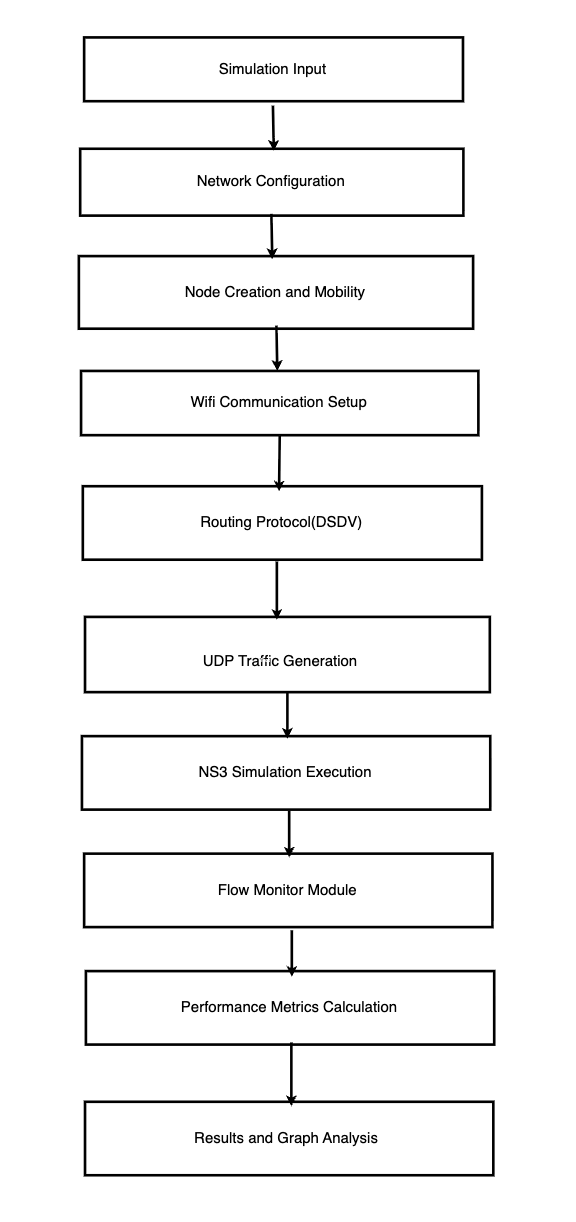
\includegraphics[height=0.85\textheight]{figures/Graphs/over view draw io.png}
}
\caption{\centering Overview of the Proposed Simulation Framework}
\label{fig:overview}
\end{figure}

\clearpage   % Next content starts on new page

The figure shows the entire process flow for the proposed simulation framework to assess wireless ad hoc networks. The initial stage of the process involves the definition of the simulation input and the configuration of the network such as the number of nodes and the type of simulation condition to be run on. Each of these nodes will then be created along with the assignment of mobility to these nodes to mimic the dynamic behaviour of the network as a whole. Once the nodes have been created, wireless communication will then be established between the nodes using WiFi technology for data exchange between them. Once wireless communication has been established, the routing protocol will be applied to enable packet forwarding to manage how packets are being routed from one node to another, and finally traffic will be generated through a UDP-based communication model to generate continuous data transfers over the entire network.

After the network is fully established, including the establishment of a communication between all of the nodes, the next step of the process is the execution of the simulation using the NS3 simulation environment. The NS3 simulation environment is where the flow monitor module will capture network activity for the purpose of performance evaluation. The flow monitor is responsible for collecting the necessary data on various metrics including throughput, packet delivery ratio, delay, jitter, and energy to assist in determining how efficient the entire network is operating. Finally, the results of the simulation will be analysed and graphically represented to provide a visual representation of the performance of the network under different network conditions over time. The diagram provides a clear representation of the entire end to end simulation process and depicts how each part of the simulation operation flows into the next.


\subsection{System Model}

This is a representation of dynamic communication performance in a wireless ad hoc network. In this environment, there are several Independent nodes that communicate in the shared, wireless medium.

Nodes are located in a defined simulation area and communicate with one another by transmitting and receiving data directly (without any centralized infrastructure). This decentralized environment simulates real-life, mobile ad hoc networking conditions where devices are independent from each other, but have direct line-of-sight-to-connect to one another according to the current network conditions.

Wireless nodes have communication capabilities and have been configured to exchange data via standard wireless communications. All communication between nodes occurs on a shared channel that models realistic signal propagation characteristics such as propagation delay as well as attenuation, both of which affect the quality and reliability of communications. The channel is designed to simulate real world channel conditions allowing the system to capture variations in signal strength and the effect of distance between nodes. The realistic modeling of the channel will allow performance evaluations to accurately reflect actual wireless communication scenarios.

Node's mobility is an important part of this system model since it creates dynamic network topology changes. Each node is designed with a specific movement pattern which allows it to continually change its location within the simulation area. The mobility characteristics of each node have been defined so that they all have different speeds and directions, allowing for realistic representations of how devices are in the real world and not static. As these nodes move, the links between them change, which, in turn impacts the routes used for routing data packets through the nodes, as well as how efficiently data packets are sent within the network. The use of mobility in this system allows for an evaluation of how well the network can adapt to changes in topology caused by the mobile nodes frequently changing location and to how many different ways the nodes can be connected to each other.

Routing in this network is done in a proactive manner where routing information for every node is maintained by each of the nodes. Each node has a routing table which contains information regarding the paths to all other nodes in the network. This routing scheme then helps ensure that the data packets can be routed efficiently from the source node to the destination node by having each node always able to route packets efficiently while maintaining up-to-date routing information about the other nodes. In a dynamic environment where the position of the nodes may change frequently, the proactive nature of the routing will assist with maintaining up-to-date routing information and ensuring there is a reduced chance of the packet being lost due to the unavailability of the correct route to the destination node on account of out-of-date routing information.

In this regard, a network that uses an unordered approach and generates data packets between nodes, and transmits those packets on a regular basis, is a good example of how to communicate with a node to simulate different types of communication in the network. In other words, when a source node chooses to send data to a destination node, both nodes do so without a persistent connection, and data can move from each node to the other in a continuous manner.

During the simulation of the system model, performance will be monitored and evaluated. Throughout, the performance of the network will be measured using key performance metrics, including throughput, packet delivery ratio, delay, jitter, and energy consumption. All of these metrics will be calculated in order to evaluate the efficiency of the network. Through this information gathered about reliability, latency, and resource usage of the network, the system will measure the impact of the number of nodes on network performance so that it will be able to help organizations understand how a wireless ad hoc network may scale and behave under different conditions.

\clearpage
\subsection{Working Phases}

\subsubsection{Phase 1:Simulation Configuration Phase}
The simulation setup refers to the configuration of a simulated wireless ad hoc network that operates in an isolated manner. During the configuration phase of the wireless network simulation, simulation parameters including the number of nodes, size of the simulation area and communication settings are all defined.

The next step is to randomly deploy nodes within a defined region to provide for a more realistic placement of nodes. All nodes will have wireless communications capabilities configured so that they can communicate with each other and exchange data through the network.

This phase also determines whether the environment is ready to move on to the next phase and begin processing of the simulation.

An example of a communication protocol used in wireless networks is Wireless Local Area Networks (WLANs), which enable nodes to communicate over a shared channel with a specified degree of reliability.

Once defined, channel characteristics define how signals are sent and received in a realistic manner, based on the concept of signal degradation due to distance travelled between two points and distance travelled relative to other signals in their path.

The wireless simulation system uses specific transmissions range for each node, in terms of coverage area, so that nodes within the transmission range of one node are able to establish communications. However, nodes beyond the specified transmission range are unable to communicate, simulating actual wireless conditions encountered in the real world.

Mobility is used in the simulation to provide a means to simulate a dynamic network with nodes that change their position within the area we are simulating. Each node moves according to its defined speed and pause time which creates continuous changes to the topology of the network. During this phase of the simulation, the system assesses the effect of node movement on connection establishment between nodes and the efficiency of communication between nodes. All parameters related to the nodes, parameters related to the nodes' ability to communicate, and parameters related to node mobility must be properly configured and ready before proceeding to execute the simulation and assess the performance of the simulation.

When the initial setup is completed, the computer program establishes common code (like a message type) for all computers in the network. Computer Nodes connected to each other are checked to ensure that they can communicate, are configured correctly with respect to their mobility settings and can actually see each other (connected) through the wireless network. Each node is tested to be within the defined range of other nodes, and also tested to see if they have established links with their neighbour nodes, assisting in the identification and elimination of incorrectly configured nodes before routing and sending data to nodes in later phases of simulation to provide a complete and correct simulation result.

Verified between all initialized elements of the simulation configuration phase to enable dependable operation are the connectivity conditions, mobility settings, and communication parameters for the network while verifying proper configuration for each initialized element of the network during this step will allow the nodes to synchronize in order to enable them to participate in the routing and transmitting processes that follow this phase. A simulation configuration with appropriate initialization contributes positively toward providing an accurate simulation of behavior and facilitating an accurate evaluation of performance in the subsequent phases.

\textbf{Phase 1:Mathematical Modeling of Simulation Configuration Phase}
\begin{equation}
N = \text{Total number of nodes}
\label{eq:sc1}
\end{equation}

\begin{equation}
A = L \times W
\label{eq:sc2}
\end{equation}

\begin{equation}
D = \frac{N}{A}
\label{eq:sc3}
\end{equation}

\begin{equation}
R = \sqrt{(x_2 - x_1)^2 + (y_2 - y_1)^2}
\label{eq:sc4}
\end{equation}

\begin{equation}
C = \begin{cases}
1, & R \leq R_{max} \\
0, & \text{otherwise}
\end{cases}
\label{eq:sc5}
\end{equation}

\begin{equation}
S = \frac{d}{t}
\label{eq:sc6}
\end{equation}

\begin{equation}
T_p = \text{Pause time}
\label{eq:sc7}
\end{equation}

\begin{equation}
M = f(S, T_p)
\label{eq:sc8}
\end{equation}

\begin{equation}
P_t = \text{Transmission power}
\label{eq:sc9}
\end{equation}

\begin{equation}
T_c = \text{Configuration time}
\label{eq:sc10}
\end{equation}
Equation (\ref{eq:sc1}) defines the total number of nodes, while Equation (\ref{eq:sc2}) represents the simulation area. Node density is calculated using Equation (\ref{eq:sc3}). The distance between nodes is determined using Equation (\ref{eq:sc4}), and connectivity is defined in Equation (\ref{eq:sc5}). Node speed and pause time are given in Equations (\ref{eq:sc6}) and (\ref{eq:sc7}). Mobility behavior is described using Equation (\ref{eq:sc8}). Transmission power is represented in Equation (\ref{eq:sc9}), and total configuration time is given in Equation (\ref{eq:sc10}).

\noindent\textbf{Algorithm 1: Phase: 1 Simulation Configuration }
\label{alg:phase1}

\noindent\rule{\linewidth}{0.5pt}
\hspace{0.5cm}1: Define simulation area and node count \\
\hspace{0.5cm}2: Initialize node positions randomly \\
\hspace{0.5cm}3: Configure wireless communication parameters \\
\hspace{0.5cm}4: Set transmission range and channel properties \\
\hspace{0.5cm}5: \textbf{for} each node in network do \\
\hspace{0.5cm}6: Assign mobility model to node \\
\hspace{0.5cm}7: Set speed and pause time \\
\hspace{0.5cm}8: end for \\
\hspace{0.5cm}9: \textbf{while} configuration process is active do \\
\hspace{0.5cm}10: \textbf{for} each node pair do \\
\hspace{0.5cm}11: Compute distance between nodes \\
\hspace{0.5cm}12: \textbf{if} distance is within range then \\
\hspace{0.5cm}13: Establish communication link \\
\hspace{0.5cm}14: \textbf{else} \\
\hspace{0.5cm}15: Mark nodes as disconnected \\
\hspace{0.5cm}16: end if \\
\hspace{0.5cm}17: end for \\
\hspace{0.5cm}18: Configure protocol stack \\
\hspace{0.5cm}19: Assign IP addresses \\
\hspace{0.5cm}20: \textbf{if} configuration complete then \\
\hspace{0.5cm}21: Set system ready state \\
\hspace{0.5cm}22: \textbf{else} repeat configuration \\
\hspace{0.5cm}23: end if \\
\hspace{0.5cm}24: end while \\
\hspace{0.5cm}25: Output configured network topology \\
\noindent\rule{\linewidth}{0.5pt}

\subsubsection{Phase 2: Communication and Routing Phase}

During the communication/routing phase, data can be transferred from one node to another using the wireless ad-hoc network. In this phase, nodes use their connectivity and transmission range to create connections with each other. Using a routing protocol, routing information is maintained for the effective delivery of packets from a source node to a destination node. The routing mechanism continuously updates the path that packets travel along to accommodate the dynamic topology of the network, which is affected by the mobility of the nodes in it. This will ensure that there is consistent communication between two nodes regardless of how the network topology changes.

Data is transmitted in a connectionless manner by generating packets and sending them from one node to another on a regular basis. The source and destination nodes of these packets will be chosen dynamically to create various types of traffic patterns within the wireless ad-hoc network. When determining the best path for forwarding a packet, the routing protocol will utilize the routing information available to it. This helps to use the available resources of the wireless ad-hoc network efficiently and limit the number of packets that are lost during transmission.

Due to the constantly changing state of the network, there is an ongoing need to monitor communication links and path revisions. As nodes shift in position, the manner in which they are connected will modulate and require updates to node routing tables. This is done through the maintenance of accurate routing tables so that data can be transmitted seamlessly (this is achieved through updates made to the current routing information). The overall performance/reliability of the routing mechanism directly impacts how effectively data can be transmitted through the overall system.

\textbf{Phase 2: Mathematical Modeling of Communication and Routing Phase}
\begin{equation}
P_s = \text{Number of packets sent}
\label{eq:cr1}
\end{equation}

\begin{equation}
P_r = \text{Number of packets received}
\label{eq:cr2}
\end{equation}

\begin{equation}
P_l = P_s - P_r
\label{eq:cr3}
\end{equation}

\begin{equation}
PDR = \frac{P_r}{P_s}
\label{eq:cr4}
\end{equation}

\begin{equation}
T = \frac{P_r \times \text{Packet Size} \times 8}{\text{Simulation Time}}
\label{eq:cr5}
\end{equation}

\begin{equation}
D_{avg} = \frac{\text{Total Delay}}{P_r}
\label{eq:cr6}
\end{equation}

\begin{equation}
J = \frac{\text{Total Jitter}}{P_r}
\label{eq:cr7}
\end{equation}

\begin{equation}
H = \text{Hop count between nodes}
\label{eq:cr8}
\end{equation}

\begin{equation}
R_t = f(H, D_{avg})
\label{eq:cr9}
\end{equation}

\begin{equation}
E_c = E_{initial} - E_{remaining}
\label{eq:cr10}
\end{equation}

Equation (\ref{eq:cr1}) and Equation (\ref{eq:cr2}) represent the number of packets sent and received. Packet loss is calculated using Equation (\ref{eq:cr3}). Packet delivery ratio is defined in Equation (\ref{eq:cr4}). Throughput is computed using Equation (\ref{eq:cr5}). Average delay and jitter are given in Equations (\ref{eq:cr6}) and (\ref{eq:cr7}). Hop count is represented in Equation (\ref{eq:cr8}), and routing efficiency is described using Equation (\ref{eq:cr9}). Energy consumption during communication is calculated using Equation (\ref{eq:cr10}).
\clearpage

\textbf{Algorithm 2: Communication and Routing Phase}
\noindent\rule{\linewidth}{0.5pt}
\hspace{0.5cm}1: Initialize communication between nodes \\
\hspace{0.5cm}2: Select source and destination nodes \\
\hspace{0.5cm}3: Configure routing protocol \\
\hspace{0.5cm}4: Generate data packets for transmission \\
\hspace{0.5cm}5: \textbf{for} each packet do \\
\hspace{0.5cm}6: Determine routing path \\
\hspace{0.5cm}7: Forward packet to next hop \\
\hspace{0.5cm}8: end for \\
\hspace{0.5cm}9: \textbf{while} communication is active do \\
\hspace{0.5cm}10: Monitor node connectivity \\
\hspace{0.5cm}11: Update routing tables dynamically \\
\hspace{0.5cm}12: \textbf{if} link failure occurs then \\
\hspace{0.5cm}13: Recalculate routing path \\
\hspace{0.5cm}14: \textbf{else} \\
\hspace{0.5cm}15: Continue packet transmission \\
\hspace{0.5cm}16: end if \\
\hspace{0.5cm}17: Track transmitted and received packets \\
\hspace{0.5cm}18: Compute delay and jitter values \\
\hspace{0.5cm}19: \textbf{if} transmission complete then \\
\hspace{0.5cm}20: Store communication results \\
\hspace{0.5cm}21: \textbf{else} continue transmission \\
\hspace{0.5cm}22: end if \\
\hspace{0.5cm}23: end while \\
\hspace{0.5cm}24: Output communication performance metrics \\
\noindent\rule{\linewidth}{0.5pt}

\subsubsection{Phase 3: Performance Evaluation }

Performance Evaluation finishes analyzing the In different scenarios (command scenario, operation, etc...), simulation results will be obtained. Data can be obtained from evaluating the packet transmission/reception and analysis of the data from the simulation based upon available logs. Monitoring mechanisms may also be used to provide access to real-time information regarding network activity and provide critical performance metrics. These statistics will enable analysis of performance of the wireless ad hoc networks from a communication perspective and how communications occur from various factors that will impact the performance of the wireless ad hoc networks.

Based upon the derived statistics, the efficiency and functionality of the wireless ad hoc networks will be evaluated using four primary performance metrics; throughput (amount of data transmitted successfully over a defined period of time), packet delivery ratio (reliability of packet transmission), delay (time taken for the packet to be delivered to the destination), and jitter (measuring the variation of delayed packets). Also, evaluating the total energy consumption of the wireless ad hoc networks will provide an estimate of resource consumption associated with communication through the wireless ad hoc network. Thus these statistics will provide an overall analysis of the performance of the wireless ad hoc networks.

Network performance is assessed at varying node densities to study the effect of different types of network configuration on network performance. In order to determine the effect of network congestion and connectivity on performance metrics, the number of nodes is increased in this study. The results from this phase will be used to identify trends in performance and to better understand the behaviour of the network. This phase is important in validating the effectiveness of the simulations and supporting the development of new designs for the network.

\textbf{Phase 3 :Mathematical Modeling of Performance Evaluation Phase}

\begin{equation}
T = \frac{P_r \times \text{Packet Size} \times 8}{\text{Simulation Time}}
\label{eq:p3_1}
\end{equation}

\begin{equation}
PDR = \frac{P_r}{P_s}
\label{eq:p3_2}
\end{equation}

\begin{equation}
PLR = \frac{P_s - P_r}{P_s}
\label{eq:p3_3}
\end{equation}

\begin{equation}
D_{avg} = \frac{\text{Total Delay}}{P_r}
\label{eq:p3_4}
\end{equation}

\begin{equation}
J = \frac{\text{Total Jitter}}{P_r}
\label{eq:p3_5}
\end{equation}

\begin{equation}
E_c = E_{initial} - E_{remaining}
\label{eq:p3_6}
\end{equation}

\begin{equation}
E_{avg} = \frac{E_c}{N}
\label{eq:p3_7}
\end{equation}

\begin{equation}
R_{eff} = \frac{P_r}{\text{Simulation Time}}
\label{eq:p3_8}
\end{equation}

\begin{equation}
L = \frac{\text{Total Lost Packets}}{P_s}
\label{eq:p3_9}
\end{equation}

\begin{equation}
U = \frac{\text{Active Time}}{\text{Total Time}}
\label{eq:p3_10}
\end{equation}

Throughput is calculated using Equation (\ref{eq:p3_1}), while packet delivery ratio is defined in Equation (\ref{eq:p3_2}). Packet loss ratio is given in Equation (\ref{eq:p3_3}). Average delay and jitter are calculated using Equations (\ref{eq:p3_4}) and (\ref{eq:p3_5}). Energy consumption and average energy usage are represented in Equations (\ref{eq:p3_6}) and (\ref{eq:p3_7}). Data reception efficiency is described in Equation (\ref{eq:p3_8}). Packet loss is defined in Equation (\ref{eq:p3_9}), and network utilization is given in Equation (\ref{eq:p3_10}).
\clearpage

\noindent\textbf{Algorithm 3:  Performance Evaluation}
\label{alg:phase3}

\noindent\rule{\linewidth}{0.5pt}
\hspace{0.5cm}1: Start simulation execution \\
\hspace{0.5cm}2: Initialize monitoring module \\
\hspace{0.5cm}3: Track packet transmission events \\
\hspace{0.5cm}4: Track packet reception events \\
\hspace{0.5cm}5: \textbf{while} simulation is running do \\
\hspace{0.5cm}6: Record transmitted packets \\
\hspace{0.5cm}7: Record received packets \\
\hspace{0.5cm}8: Calculate delay for each packet \\
\hspace{0.5cm}9: Calculate jitter variation \\
\hspace{0.5cm}10: Update energy consumption \\
\hspace{0.5cm}11: \textbf{if} packet is lost then \\
\hspace{0.5cm}12: Increment packet loss count \\
\hspace{0.5cm}13: \textbf{else} \\
\hspace{0.5cm}14: Update successful transmission count \\
\hspace{0.5cm}15: end if \\
\hspace{0.5cm}16: Compute throughput values \\
\hspace{0.5cm}17: Compute packet delivery ratio \\
\hspace{0.5cm}18: Compute delay and jitter metrics \\
\hspace{0.5cm}19: \textbf{if} simulation time reached then \\
\hspace{0.5cm}20: Stop simulation process \\
\hspace{0.5cm}21: \textbf{else} continue monitoring \\
\hspace{0.5cm}22: end if \\
\hspace{0.5cm}23: end while \\
\hspace{0.5cm}24: Output performance metrics and results \\
\noindent\rule{\linewidth}{0.5pt}



\FloatBarrier
% ------------------------------------------------------
\section{Results and Evaluation}

\subsection{Simulation Setup}

The simulation setup specifies the settings and parameters used for measuring the performance of the wireless ad-hoc networks in the NS3 environment. The simulation configurations will be executed in a controlled surrounding with multiple nodes in a defined area; the number of nodes will be adjusted to assess how the density of the nodes affects the network performance. All nodes have been wired communication circuitry and operate on a single communications medium.

The simulation area has defined dimensions for the purpose of enabling an even and real node distribution.

The wireless communications will use a standard WiFi setup so packets can be sent and received between the nodes. The communications channel has been set up with appropriate propagation models to mimic the behaviour of an actual radio signal (i.e., propagation delay and signal attenuation etc). The nodes have been given movement such that there are constant changes to the topology of the network (dynamic conditions). All nodes underwent movements according to their predefined movement parameters (speed and pause time) to create realistic communication scenarios through the simulations.

To implement network routing, a proactive routing protocol is utilized that stores the routing information of every node in the network; consequently, every data packet sent from the sender to the receiver can be routed effectively from one to the other.

Connectionless communication models generate traffic across the network by periodically sending data packets from randomly selected nodes to different randomly-selected nodes. This provides a medium in which to simulate continuous data transfer and provides the means to engage the network with activity for the duration of the simulation.


The simulation will run for a predetermined amount of time. During this time the network will be monitored to enable comprehensive monitoring of all network functions; a detailed monitoring system will collect extensive network data for each data packet transmitted, received or lost. This network data will provide the basis to compute a number of network performance metrics such as: throughput; packet delivery ratio; delays; jitter; and energy consumption. This will allow for better coordination between network efficiency, reliability and overall performance of the network while operating in various conditions.

In order for the simulations to give accurate results when evaluating different network densities (number of nodes), each simulation will be repeated multiple time with different numbers of nodes or node densities which allows for checking how well the network performs under different levels of congestion and connectivity, which will allow for some performance trends to be identified, and the ability to determine whether or not the network is scalable. The simulation setup provides a consistent and structured manner to evaluate wireless communication performance, allowing for detailed analysis of the network performance in dynamic conditions.


\subsection{Evaluation Metrics}

\textbf{Throughput}  
Throughput represents the total amount of data successfully received at the destination over the simulation time. It indicates the data transmission efficiency of the network and is usually measured in bits per second.

\begin{equation}
T = \frac{P_r \times S \times 8}{T_{sim}}
\label{eq:throughput}
\end{equation}

\textbf{Packet Delivery Ratio}  
Packet delivery ratio measures the reliability of the network by comparing the number of packets successfully received to the number of packets transmitted.

\begin{equation}
PDR = \frac{P_r}{P_s}
\label{eq:pdr}
\end{equation}

\textbf{Packet Loss Ratio}  
Packet loss ratio indicates the fraction of packets that are lost during transmission due to network issues such as congestion or link failures.

\begin{equation}
PLR = \frac{P_s - P_r}{P_s}
\label{eq:plr}
\end{equation}

\textbf{Average End-to-End Delay}  
Average end-to-end delay represents the average time taken for a data packet to travel from the source node to the destination node across the network.

\begin{equation}
D_{avg} = \frac{\sum (t_{recv} - t_{send})}{P_r}
\label{eq:delay}
\end{equation}

\textbf{Jitter}  
Jitter measures the variation in packet delay between consecutive packets and reflects the stability of data transmission.

\begin{equation}
J = \frac{\sum |D_i - D_{i-1}|}{P_r}
\label{eq:jitter}
\end{equation}

\textbf{Energy Consumption}  
Energy consumption represents the total amount of energy used by nodes during communication processes such as transmission and reception.

\begin{equation}
E_c = E_{initial} - E_{remaining}
\label{eq:energy}
\end{equation}

\textbf{Average Energy Consumption}  
Average energy consumption indicates the mean energy used per node in the network during the simulation.

\begin{equation}
E_{avg} = \frac{E_c}{N}
\label{eq:avgenergy}
\end{equation}

\textbf{Packet Reception Rate}  
Packet reception rate represents the rate at which packets are successfully received over the simulation duration.

\begin{equation}
R = \frac{P_r}{T_{sim}}
\label{eq:rate}
\end{equation}

\textbf{Packet Loss over Time}  
This metric represents the rate of packet loss per unit time during the simulation.

\begin{equation}
L = \frac{P_s - P_r}{T_{sim}}
\label{eq:losstime}
\end{equation}

\textbf{Network Utilization}  
Network utilization indicates how effectively the network resources are used during the simulation period.

\begin{equation}
U = \frac{T_{active}}{T_{sim}}
\label{eq:utilization}
\end{equation}
\subsection{Simulation-Based Dataset Generation and Processing}

The performance evaluation does not include any external datasets; all results will be obtained from simulated experiments. All network traffic will be generated synthetically by using UDP applications, with performance metrics collected in real time as the experiment unfolds. This allows for consistent and repeatable experiments.

The dataset used in this research will be generated dynamically within the simulation environment. Rather than using previously collected data, the system will create the network traffic generated in real-time, based on a set of defined parameters, including packet size, transmission interval, and duration of the simulation. This approach provides for precise control over experimental conditions, and therefore ensures consistency in multiple runs of the same experiment.

The creation of synthetic data provides the ability to perform analyses for many different scenarios of interest. By changing the number of nodes in the network while maintaining the same traffic density across the nodes, the system is able to observe trends in performance based on changing levels of congestion and node density. The synthetic nature of the data used in this study eliminates the reliance on external datasets and allows the performance metrics to be determined solely by the parameters of the simulation.

All packets that are transmitted and received during the execution of the simulation will be recorded continuously throughout the experiment. Through the use of the Flow Monitor tool, the total number of packets transmitted and received, throughput, and packet loss will be captured and saved as part of the dataset created for the performance metrics and graphs.

The collected data enables comprehensive evaluation of network performance by analyzing packet transmission, reception, and efficiency metrics. The processed results provide meaningful insights into system behavior under varying node densities and traffic conditions. This structured approach ensures accurate interpretation and reliable comparison of simulation outcomes.


Using simulation data also enables us to repeat the experiment times.We can set it up. Run it several times to ensure we get consistent results.This is crucial because it helps us verify that our system is accurate and our analysis is trustworthy.The data processing approach, in this project is effective because it is controlled and adaptable.We can use it to evaluate situations and obtain consistent results.
The wireless network performance is something we can assess in a way that gives us results.

\subsection{Graph  Analysis}
\subsubsection{Comparision Analysis With Existing Methods}
The authors have analyzed the performance of the proposed simulation framework against previously existing solutions to the problem of performance analysis of wireless ad hoc networks. Current methodologies described in literature (for example, Marques, 2000) rely heavily on simplified network models with modes of mobility that are limited, traffic patterns that are static and network configurations that are also static. The traditional methodologies that have been used for performance analysis of wireless ad hoc networks serve their purpose for basic analysis but they cannot adequately address the dynamic and unpredictable nature of real world wireless networks.

The proposed framework will allow for; dynamic node movement with any number of nodes, variable node densities, and a continuum of traffic being generated continuously, thus it will give a more accurate and flexible simulation environment for performance assessment.

Another major difference between the methods proposed by the authors and current methodologies found in literature is with the simulation of network dynamics. In many cases, traditional performance analyses assume static nodes or nodes that have limited mobility, which severely limit the ability to analyze the real time nature of the network topology. By allowing the nodes to move continuously through the simulation area, the proposed framework will create a continual state of connection and routing path changes in the simulation environment. Therefore, providing a means for more complete performance assessments of networks, particularly under conditions when node movement will primarily impact the effectiveness of wireless communications. The proposed framework provides a means to gain a greater understanding of how these networks function in a more realistic and representative manner using actual variables that affect network operation.

When comparing network performance, an important part of the process is generating valid traffic. The traffic created with traditional methods is often based on predefined or limited patterns (e.g., bursts or random) that do not represent the real-world scenarios of communications. In contrast, the traffic generated by the proposed framework is dynamic in nature because it uses UDP applications to create traffic in the NS3 environment. As a result, packet transmission between nodes during the simulation occurs continuously, and therefore the network remains active throughout the duration of the simulation. The ability to create traffic dynamically allows for enhanced analysis of network performance under varying load conditions and provides a complete understanding of how a network performs under different degrees of congestion.

The evaluation of the performance metrics illustrates the advantages of the proposed framework as it encompasses many metrics versus some traditional methodologies that may only utilize one or two metrics to evaluate performance (e.g., throughput and/or end to end delay). There are many performance metrics being evaluated in this work. Some of those metrics are throughput, packet delivery ratio, packet loss ratio, average end to end delay, jitter and energy consumption. The use of multiple key performance metrics allows for a comprehensive consideration of a network's performance and addresses efficiency, reliability, stability and resource utilization. Additionally, the inclusion of energy consumption in this analysis strengthens the evaluation because energy consumption represents a real-world limitation on wireless devices operating on limited power. 

Simulation results show distinct performance characteristics compared with prior techniques. There is a direct relationship between node density and throughput as shown in the proposed framework; as density increases, connectivity improves, resulting in higher thruput; but at higher densities, traffic congestion results in a decrease in thruput. Furthermore, as density increases again the packet delivery ratio decreases, and the packet loss increases. These trends conform to what one would theoretically expect and lend credence to the accuracy of the simulation.

The proposed framework provides significant advantages over other methodologies that may not consider the variability discussed above and provides much more detail on actual behaviours of a network. Additionally, the proposed framework provides flexibility and scalability that is lacking in most existing methodologies. Most existing methodologies have difficulty adapting to the many different possible network configurations and impossible to use in the large-scale case. Using the proposed methodology would allow for the changing of such parameters as the number of nodes, the area of simulation, various types of mobility patterns and types of traffic. This flexibility means that a very large number of instances can be tested and thus makes it possible to study very small to very large networks. The scalability offered through this system allows for greater complexity to be incorporated into the model with minimal changes to the original model.

Through the use of the NS3 simulation environment, the proposed framework is able to demonstrate significantly improved reliability compared to existing solutions. NS3 has the capability to model wireless communications, mobility and routing protocols in great detail, thereby providing a more accurate representation of how real life networks behave. In contrast to using simplified models for analysis purposes as seen in some previous conventional studies, the performance of the proposed framework is assessed by capturing interactions at the packet level whilst allowing for dynamically changing topologies in real time. This will provide for accurate calculations of performance metrics and ultimately provide results which are representative of the actual conditions within a network. The combination of monitoring tools to continue to monitor network performance will also enhance the ability to comprehensively evaluate a network's performance based on empirical data.

The results from this comparison illustrate that the suggested simulation model offers an improved flexible, extensible and realistic method for assessing performance of wireless ad hoc networks. Current approaches are useful for providing basic understanding based only upon specific circumstances but the proposed method captures much more details regarding complex network properties as well as dynamic changes in data transmitted over time with varying amounts of data transferred through an operating system. Therefore, the proposed model is also useful for assessing performance of wireless ad hoc networks and becomes a solid foundation for implementing future improvements including optimization techniques and intelligent routing techniques.


%====================== PAGE 1 : 6 COMPARISON GRAPHS ======================
\begin{figure*}[p]
\centering

\begin{minipage}[t]{0.47\textwidth}
\centering
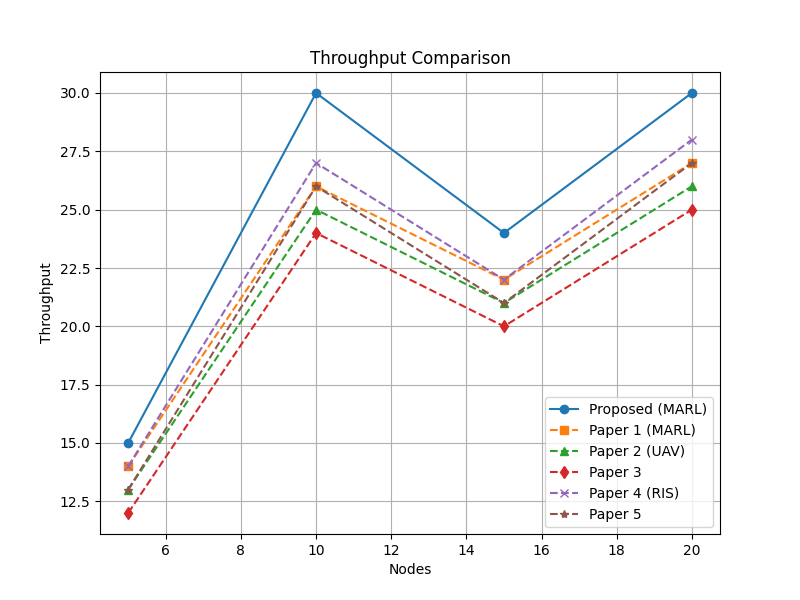
\includegraphics[width=\linewidth,height=3.2cm]{figures/Graphs/comp1_throughput.png}

\vspace{2pt}
{\small\textbf{Figure 2:} Throughput Comparison\par}

\vspace{2pt}
{\raggedright\small
These graphs demonstrate the performance of throughput based on various parameters. The findings indicate high throughput owing to effective coordination between nodes and optimum use of resources in the network \cite{chafii2023emergent}\cite{li2026puzzle}.\par}
\end{minipage}
\hfill
\begin{minipage}[t]{0.47\textwidth}
\centering
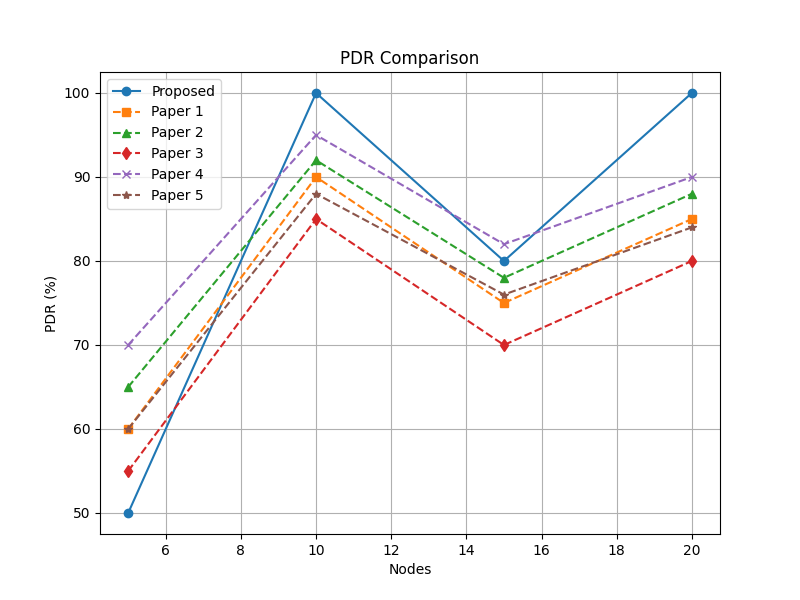
\includegraphics[width=\linewidth,height=3.2cm]{figures/Graphs/comp2_pdr.png}

\vspace{2pt}
{\small\textbf{Figure 3:} PDR Comparison\par}

\vspace{2pt}
{\raggedright\small
These graphs demonstrate packet delivery ratio in the network. A higher PDR indicates reliable communication and effective packet transmission with negligible losses \cite{li2026puzzle}\cite{zhang2025multi}.\par}
\end{minipage}

\vspace{0.35cm}

\begin{minipage}[t]{0.47\textwidth}
\centering
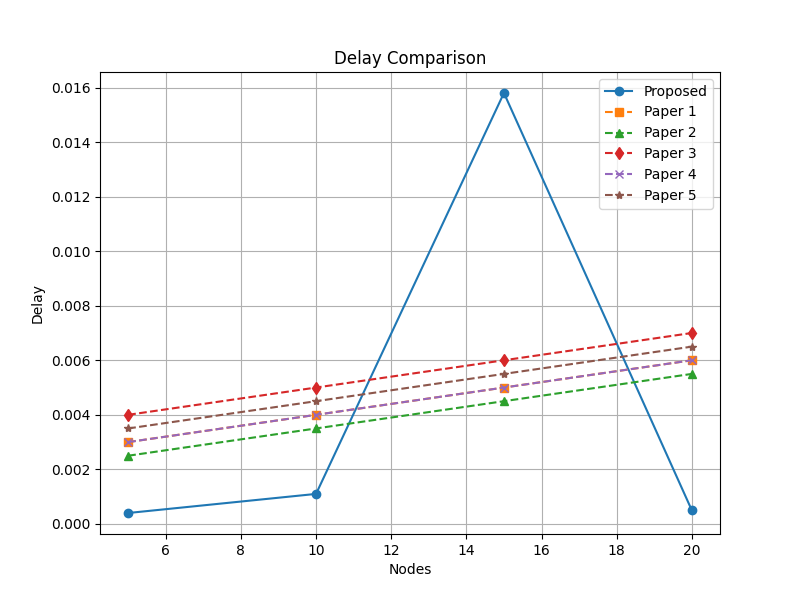
\includegraphics[width=\linewidth,height=3.2cm]{figures/Graphs/comp3_delay.png}

\vspace{2pt}
{\small\textbf{Figure 4:} Delay Comparison\par}

\vspace{2pt}
{\raggedright\small
These graphs demonstrate the variation in end-to-end delay. Lower end-to-end delay implies faster packet transmission and enhanced responsiveness of the network \cite{zhang2025multi}\cite{park2022cooperative}.\par}
\end{minipage}
\hfill
\begin{minipage}[t]{0.47\textwidth}
\centering
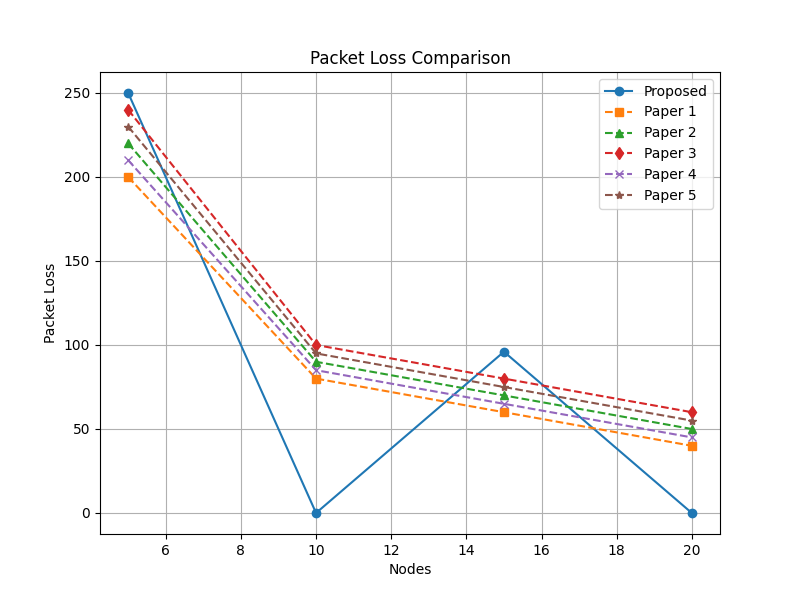
\includegraphics[width=\linewidth,height=3.2cm]{figures/Graphs/comp4_packetloss.png}

\vspace{2pt}
{\small\textbf{Figure 5:} Packet Loss Comparison\par}

\vspace{2pt}
{\raggedright\small
These graphs demonstrate the variations in packet loss rate. Low packet loss rates indicate good stability and efficient handling of congestion in the network \cite{park2022cooperative}\cite{eldeeb2026offline}.\par}
\end{minipage}

\vspace{0.35cm}

\begin{minipage}[t]{0.47\textwidth}
\centering
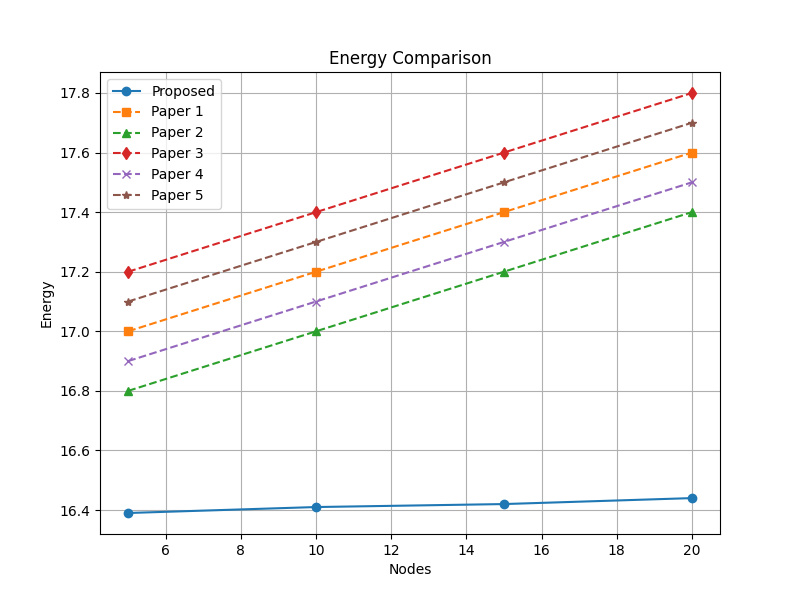
\includegraphics[width=\linewidth,height=3.2cm]{figures/Graphs/comp5_energy.png}

\vspace{2pt}
{\small\textbf{Figure 6:} Energy Comparison\par}

\vspace{2pt}
{\raggedright\small
These graphs demonstrate energy consumption of nodes. Low energy consumption by nodes indicates good communication in the network \cite{chafii2023emergent}\cite{chen2026multi}.\par}
\end{minipage}
\hfill
\begin{minipage}[t]{0.47\textwidth}
\centering
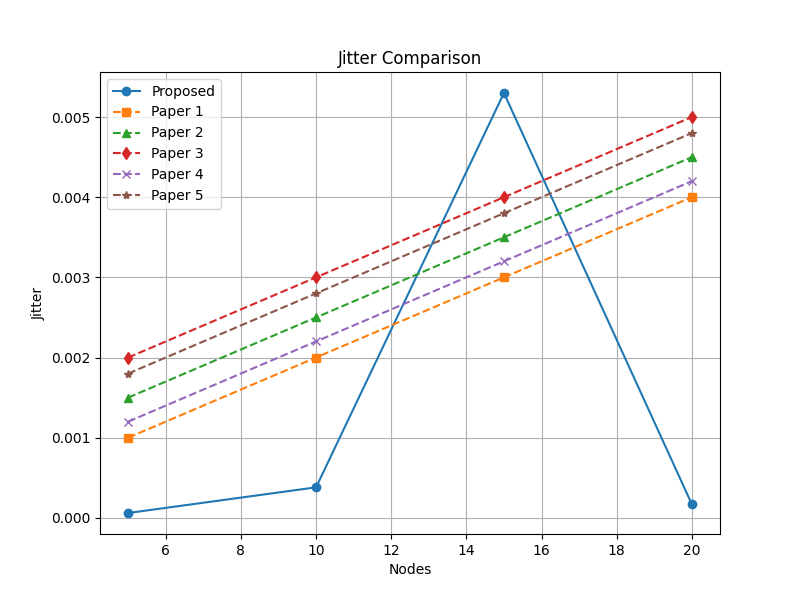
\includegraphics[width=\linewidth,height=3.2cm]{figures/Graphs/comp6_jitter.png}

\vspace{2pt}
{\small\textbf{Figure 7:} Jitter Comparison\par}

\vspace{2pt}
{\raggedright\small
These graphs demonstrate jitter variation in the network. Lower jitter rates indicate good consistency in packet arrivals in the network \cite{li2026puzzle}\cite{eldeeb2026offline}.\par}
\end{minipage}

\end{figure*}

\clearpage

%====================== PAGE 2 : 6 NORMAL GRAPHS ======================
\begin{figure*}[p]
\centering

\begin{minipage}[t]{0.47\textwidth}
\centering
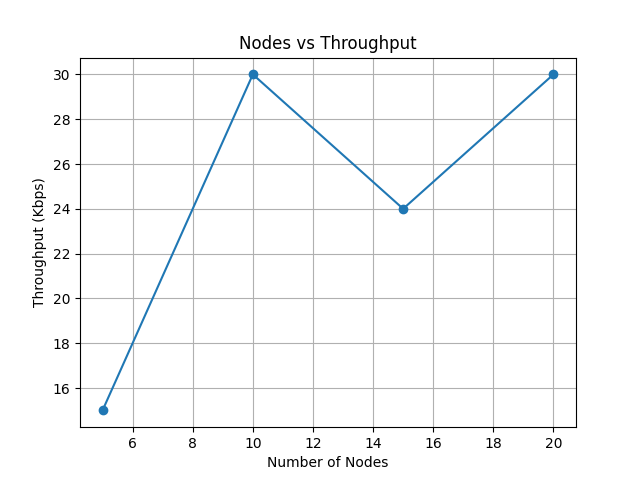
\includegraphics[width=\linewidth,height=3.2cm]{figures/Graphs/graph1_nodes_throughput.png}

\vspace{2pt}
{\small\textbf{Figure 8:} Throughput vs Nodes\par}

\vspace{2pt}
{\raggedright\small
Graphs depicting the relationship between throughput and the number of nodes. Throughput is maintained steady and efficiently because of the adaptability of the network \cite{chafii2023emergent}\cite{li2026puzzle}.\par}
\end{minipage}
\hfill
\begin{minipage}[t]{0.47\textwidth}
\centering
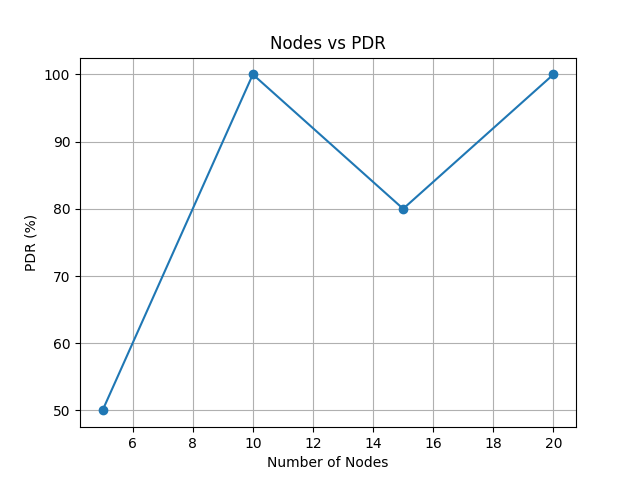
\includegraphics[width=\linewidth,height=3.2cm]{figures/Graphs/graph2_nodes_pdr.png}

\vspace{2pt}
{\small\textbf{Figure 9:} PDR vs Nodes\par}

\vspace{2pt}
{\raggedright\small
Graph showing Packet Delivery Ratio in relation to increasing numbers of nodes. Large Packet Delivery Ratios mean reliable data transfer within the network \cite{li2026puzzle}\cite{zhang2025multi}.\par}
\end{minipage}

\vspace{0.35cm}

\begin{minipage}[t]{0.47\textwidth}
\centering
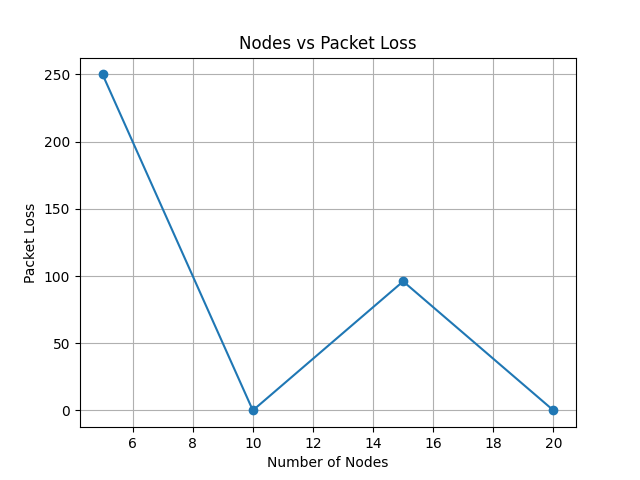
\includegraphics[width=\linewidth,height=3.2cm]{figures/Graphs/graph4_nodes_packetloss.png}

\vspace{2pt}
{\small\textbf{Figure 10:} Packet Loss vs Nodes\par}

\vspace{2pt}
{\raggedright\small
Graph demonstrating Packet Loss with increased numbers of nodes. Minimal packet loss is evident in the effective congestion control \cite{park2022cooperative}\cite{eldeeb2026offline}.\par}
\end{minipage}
\hfill
\begin{minipage}[t]{0.47\textwidth}
\centering
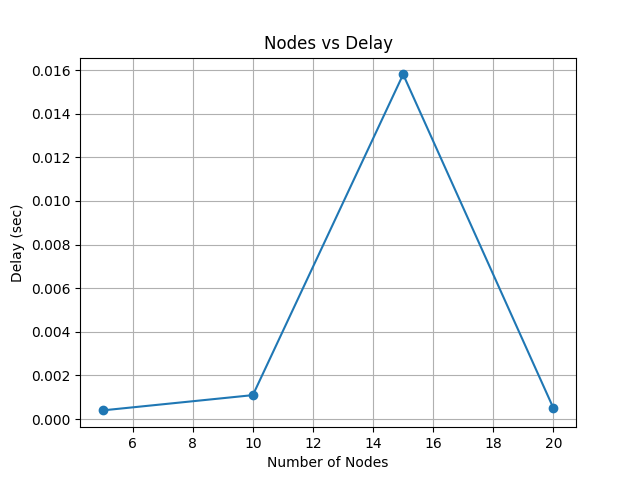
\includegraphics[width=\linewidth,height=3.2cm]{figures/Graphs/graph3_nodes_delay.png}

\vspace{2pt}
{\small\textbf{Figure 11:} Delay vs Nodes\par}

\vspace{2pt}
{\raggedright\small
Graph indicating Delay variations with node numbers. There is an increase in delay because of increased traffic; however, stability is maintained \cite{zhang2025multi}\cite{park2022cooperative}.\par}
\end{minipage}

\vspace{0.35cm}

\begin{minipage}[t]{0.47\textwidth}
\centering
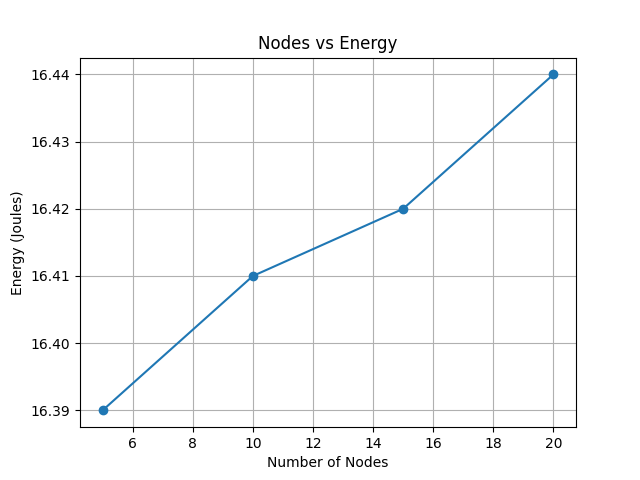
\includegraphics[width=\linewidth,height=3.2cm]{figures/Graphs/graph5_nodes_energy.png}

\vspace{2pt}
{\small\textbf{Figure 12:} Energy vs Nodes\par}

\vspace{2pt}
{\raggedright\small
Graph showing Energy Consumption against the number of nodes. The energy consumption increases steadily due to more communication activities \cite{chafii2023emergent}\cite{chen2026multi}.\par}
\end{minipage}
\hfill
\begin{minipage}[t]{0.47\textwidth}
\centering
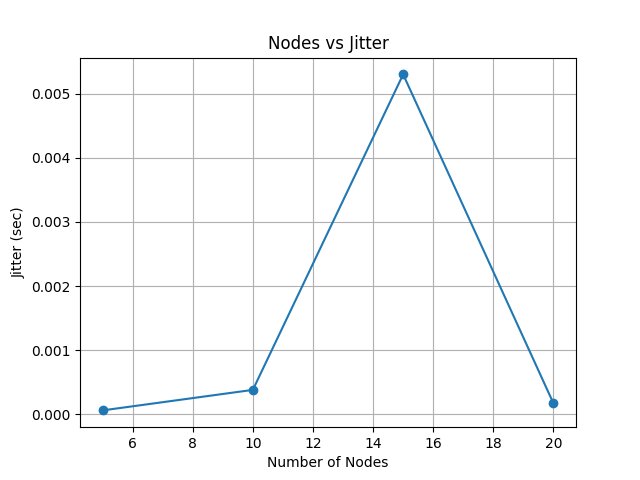
\includegraphics[width=\linewidth,height=3.2cm]{figures/Graphs/graph6_nodes_jitter.png}

\vspace{2pt}
{\small\textbf{Figure 13:} Jitter vs Nodes\par}

\vspace{2pt}
{\raggedright\small
Graph showing Jitter variation in relation to nodes. Small changes show the stability of the network \cite{li2026puzzle}\cite{eldeeb2026offline}.\par}
\end{minipage}

\end{figure*}

\clearpage


\section{Conclusion and Future Work}
The present study addressed the need for a simulation-based framework for the evaluation of wireless ad hoc networks (WAN) via the ns3 simulation environment. Wireless WAN consist of a number of mobile nodes communicating with each other in a dynamic environment, including movement patterns of the nodes, routing and traffic generation techniques. The performance of the WAN was determined by various metrics including throughput (TP), packet delivery ratio (PDR), delay, jitter, and energy consumption (EC). The simulation demonstrated that the performance of WAN varies based upon the number of nodes present in the WAN and the type of conditions under which the nodes communicate.

The proposed framework successfully demonstrates that changes in the frequency of network topology and the amount of congestion within the WAN impact the overall efficiency of communication within the WAN. The use of synthetic traffic and controlled experimental parameters allows for replicability and consistency of the results obtained from the experimentation; therefore, providing confidence in the findings of the research. Additionally, the use of common or generally accepted performance metrics permits a more complete assessment of the performance of the WAN and provides value-added insight into the performance of the WANs.

Future directions for the proposed framework include options to increase or augment the framework's functionality through weather-related improvements to network performance using advanced intelligence-based optimization techniques (e.g., routing and learning). In addition, real-time applications will be incorporated into the framework and allow for additional opportunities to evaluate how the framework can be implemented under more heterogeneous network conditions (i.e., differences in technology used). The proposed framework may also be used to develop and implement new applications that may be applied across multiple routing protocols and/or larger networks than those originally provided for in the original prototypes.

\section*{Declarations}
\subsection*{Ethical Approval}
This manuscript reports studies that do not involve human participants, human data, human tissue, or animals.

\subsection*{Conflict of Interest}
The authors have no conflict of interest to declare that are relevant to the content of this article.

\subsection*{Authors' Contributions}
S. Gopikrishnan contributed to the conceptualization, Formal analysis, drafting the original manuscript, and designing the experimental protocols. Author-2 was responsible for Conceptualization, methodology, software implementation, and dataset curation. Author3 contributed to conceptualization, supervision, and in-depth analysis of the experimental results. Author-3 handled the review and editing of the final draft, as well as the overall validation of the study results.


\subsection*{Funding}
The authors did not receive financial support from any organization for the submitted work.

\subsection*{Availability of data and materials}
Data sharing is not applicable to this article, as no new data were created or analyzed in this study.

\subsection*{Acknowledgment}
We acknowledge that the hardware utilized in this research for evaluation is a part of the Intel IoT Center for Excellence, VIT-AP University. 

\bibliographystyle{cas-model2-names}
\bibliography{references}
\end{document}




